\documentclass[
    a4paper,
    twocolumn,
]{article}

% Table insertions
% --------------------------------------------------
\usepackage{graphics}

% Image insertions
% --------------------------------------------------
\usepackage{graphicx}
\usepackage[belowskip=-3pt,aboveskip=8pt]{caption}
\graphicspath{{./images/}}

% Input and font encoding
% --------------------------------------------------
\usepackage[utf8]{inputenc}
\usepackage[T1]{fontenc}

% biblatex --- Bibliography setup
% --------------------------------------------------
\usepackage[
    backend=biber,
    style=numeric,
    sorting=none,
]{biblatex}

\addbibresource{sources.bib}

% hyperref --- Hyperlinks in PDF
% --------------------------------------------------
\usepackage[pdfusetitle]{hyperref}

% Set colors of links
\hypersetup{
    colorlinks=true,
    linkcolor=magenta,
    citecolor=,
    urlcolor=blue,
}

% Allow line-breaks in links and URLs
\hypersetup{breaklinks=true}

% Use the normal document font for URLs rather than monospace
\urlstyle{same}

% Document Metadata
% --------------------------------------------------
\title{INF3200: Mandatory Assignment 2}
\author{Yasiru Rathsara Witharanage}
\date{\today}

% Document
% --------------------------------------------------
\begin{document}

\maketitle

\begin{abstract}
    \textbf{In the context of distributed systems, the term stability is trivial as the existence of individual nodes are not predefined and fixed. Hence it is significantly important to address the issue of inconsistent structure dynamically while minimizing the adverse impact on performance of the system thus providing transparency to the end-user. This paper discusses a solution to this complication of ever-changing participants of a key-value store based on chord~\cite{1} along with the experiments conducted to measure its performance and behavior.}
\end{abstract}

\section{Introduction}

In this study, a distributed hash table was implemented based on chord which uses a ring topology where each node in the system is only aware of its predecessor and successor initially. A node is responsible for storing and retrieving of any key-value pair that belongs to its bucket space based on node id. These keys and node ids are first hashed using SHA256~\cite{2} algorithm in order to minimize the collision of two separate nodes and to utilize the potential of supporting an enormously large distributed store.\\

Main objective of this study is to build a chord network resilient to dynamic changes which can be occurred due to joining and leaving of nodes. This adaptation also includes coping against crashing of nodes without any prior notification and re-construct network leaving these out-of-reach nodes. Moreover, it should be able to detect these left out nodes and include them in the network whenever they are reachable again.\\

Following HTTP endpoints are exposed to serve store functionalities as well as to cope with dynamically changing structure of server nodes. Note that nodes are not aware of cluster information and cluster-info endpoint circulates an HTTP request around the ring structure to collect necessary data. 

\begin{itemize}
	\item PUT /storage/key - stores a value provided in the raw body
	\item GET /storage/key - returns the value of a key (returned in raw body)
	\item POST /join?nprime=HOST:PORT - joins the network using an existing node
	\item POST /leave - leaves out the requested node from network
	\item GET /neighbors - returns neighbours of a node
	\item GET /node-info - returns a JSON response of requested node information
	\item GET /cluster-info - returns cluster information
\end{itemize}

\section{Project Description}
\subsection{Design}

Each individual node in the network is given an id based on the SHA256 hash value of its own hostname and is only aware of its neighbours, i.e. predecessor and successor. Whenever a query is received by a node, it initially checks whether the requested key belongs to itself and if not, it proceeds to the immediate successor. This process is iterated until the correct node for key is discovered and the corresponding response is returned along the same route.

When joining the network, a request is sent to the new node along with an existing node in the cluster and thus a join is initiated to this entry point where it starts circulating the request until the corresponding successor of new node is reached. This successor then updates its new predecessor while notifying the ex-predecessor to update its successor. Once this circulation is successful, neighbors of the new node will be returned by the response and updated in the joining node.\\

On the other hand, a node notifies both its predecessor and successor upon leaving, to update their neighbors accordingly. Since these two requests are independent of each other, they can be executed in parallel thus saving an overhead latency of multiple requests. In both these scenarios, bucket space will be adjusted with respect to the network change. \\

Moreover, a probing mechanism is implemented in each node with a configured timeout to detect any out of reach condition of its predecessor and automatically rectify with active nodes by eliminating the crashed node. Once a crash is recognized, the successor will circulate an internal HTTP request until the last active node is found and thus updating a new connection between these two nodes. Immediate successors also keep track of these disconnected nodes to add once they become reachable again and this check is done in the order of proximity, i.e. closest lost node will be checked before the rest and so on. However, this system does not support the migration of existing key-value pairs when changing the components of network.

\subsection{Implementation}

Golang was used for the implementation of chord with a flat-hierarchical code structure and different layers for each functionality. HTTP endpoints listed previously were implemented in HTTP layer while node layer contains details (node id, predecessor, successor) related with the node along with validating key function. SHA256 was used for hashing of both key and node id to match with relevant buckets. All the outgoing HTTP requests to neighbors are implemented in neighbor layer and An HTTP client was used to proceed any request with a key that does not belong to the corresponding node. All key-value entry pairs are stored in an in-memory map which is specifically designed for concurrent use.\\

A sample set is given below for the configuration values of parameters required by the implementation but however user is allowed to provide his own desired values for service configurations. 

\begin{verbatim}
# service configs
port: 52520
request_timeout_sec: 5
ttl_min: 180

# neighbor configs
probe_interval_sec: 10
detect_crash_timeout_sec: 2

# logger configs
colors_enabled: true
log_level: "TRACE"
file_path: true
\end{verbatim}

\texttt{request\_timeout\_sec} refers to the waiting time of a single HTTP request by a node in seconds and each node has a TTL in minutes for the self-termination configured by \texttt{ttl\_min}. \texttt{probe\_interval\_sec} is used as the time interval in which each node is checking if their immediate predecessors are reachable. A separate HTTP client is used to detect whether a successor is not responsive in finding the last active node triggered by a node crash. This detection is done with a timeout configured by \texttt{detect\_crash\_timeout\_sec}. \\

Responses of all endpoints except for node-info are returned as raw body since unmarshalling operation in golang is quite expensive and doing this in every node per request will be tedious. Instead, conversion of byte array directly into string for further processing was used thus saving the overhead. \\

Go HTTP server implicitly uses different go-routines per each request hence use of mutex locks were required when updating states of neighbors in each node. It is assumed that host names are always in the correct form but however, a regex can be added for validation if required.

\section{Evaluation}

Several experiments were carried out to evaluate performance and stability of network with dynamic changes in the structure. Table 1 provides details about sets of nodes used and hardware specifications of them.

\begin{table}[!ht]
	\renewcommand{\arraystretch}{1.4}
	\centering
	\resizebox{\columnwidth}{!}{%
		\begin{tabular}{|c | c | c | c | c | c|} 
			\hline
			Nodes & Model & CPUs & Cores & Processors & RAM (GB)\\
			\hline
			1-29  & Lenovo P310 & 1 & 4 & 4 & 32 (4x8GB)\\ 
			\hline
			30-37  & Lenovo M910s & 1 & 4 & 4 & 32 (2x16GB)\\ 
			\hline
			38-50 & Lenovo m93p & 1 & 4 & 8 & 16 (2x8GB) \\ 
			\hline
		\end{tabular}%
	}
	\caption{Hardware specification of nodes}
\end{table}

First experiment was conducted to measure the time consumption of network to stabilize after different number of joins of nodes in each test attempt. This was achieved by sending sequential join requests to every initialized node (but not connected) and logging timestamps with each node's action. Total time to stabilize was taken as the time difference between initial join action and the last neighbor update by a node. Finally cluster information response was considered to ensure that the network consisted of desired number of nodes.\\

A similar experiment was conducted to measure stability of network upon leaving of nodes. In this experiment, different number of nodes were initialized and connected after which a half of the joined nodes were requested to leave. These messages were sent sequentially to nodes and total time for stabilization was calculated as before (time difference between initial leave request and last neighbor update).\\

Finally, adaptation of network on crashing of nodes without any prior notification was evaluated as well. In this experiment, crash requests were sent in parallel as a burst after initializing 50 connected nodes in each attempt and time for stabilization was measured as the time difference between initial detection of crash and final log of the successor of a crashed node. To this end, additional logs were implemented in nodes such that it outputs timestamps when a crash is detected initially and after fixing a crashed node by re-establishing a new connection with last active node.

\section{Results}

Following are the average stabilization times taken for the above experiments in seconds by varying the number of nodes. Average times were calculated after carrying out each test scenario at least 3 times.\\

\begin{table}[!ht]
\renewcommand{\arraystretch}{1.4}
\centering
\resizebox{\columnwidth}{!}{%
	\begin{tabular}{|c | c | c | c|} 
		\hline
		Type & Initial nodes & Nodes joined/left/crashed & Average time (s) \\
		\hline
		join & 0 & 10 & 0.234366 \\
		\hline
		join & 0 & 20 & 0.577214 \\
		\hline
		join & 0 & 30 & 1.01368 \\
		\hline
		join & 0 & 40 & 1.431316 \\
		\hline
		join & 0 & 50 & 1.867544 \\
		\hline
		leave & 10 & 5 & 0.072111 \\
		\hline
		leave & 20 & 10 & 0.156652 \\
		\hline
		leave & 30 & 15 & 0.252503 \\
		\hline
		leave & 40 & 20 & 0.317286 \\
		\hline
		leave & 50 & 25 & 0.408408 \\
		\hline		
	\end{tabular}%
}
\caption{Results of experiment 1 and 2 with average times for stabilization}
\end{table}

Note that time measured in third experiment is taken after stabilization of all partitioned networks and also includes a timeout configured as 1 second in detecting the last active node. An initial size of 50 connected nodes was considered in each test attempt of crashing.

\begin{table}[!ht]
	\renewcommand{\arraystretch}{1.4}
	\centering
	\resizebox{\columnwidth}{!}{%
		\begin{tabular}{|c | c | c | c|} 
			\hline
			Nodes crashed & Average time (s) & Corrected Average time (s) \\
			\hline
			1 & 6.048608 & 5.048608 \\
			\hline
			2 & 6.536561 & 5.536561 \\
			\hline
			3 & 6.489625 & 5.489625 \\
			\hline
			5 & 6.804467 & 5.804467 \\
			\hline
			10 & 6.780120 & 5.780120 \\
			\hline		
		\end{tabular}%
	}
	\caption{Results of experiment 3 with average times for stabilization}
\end{table}

\section{Discussion}

Figure 1 below shows the average times taken for stabilization of experiment 1 and 2 (join and leave respectively) in seconds with error bars for standard deviation~\cite{3}. It is also assumed that latency incurred by logging operations are negligible when compared to the above measured average times.

\setlength{\intextsep}{10pt plus 2pt minus 0pt}
\begin{figure}[!ht]
	\centering
	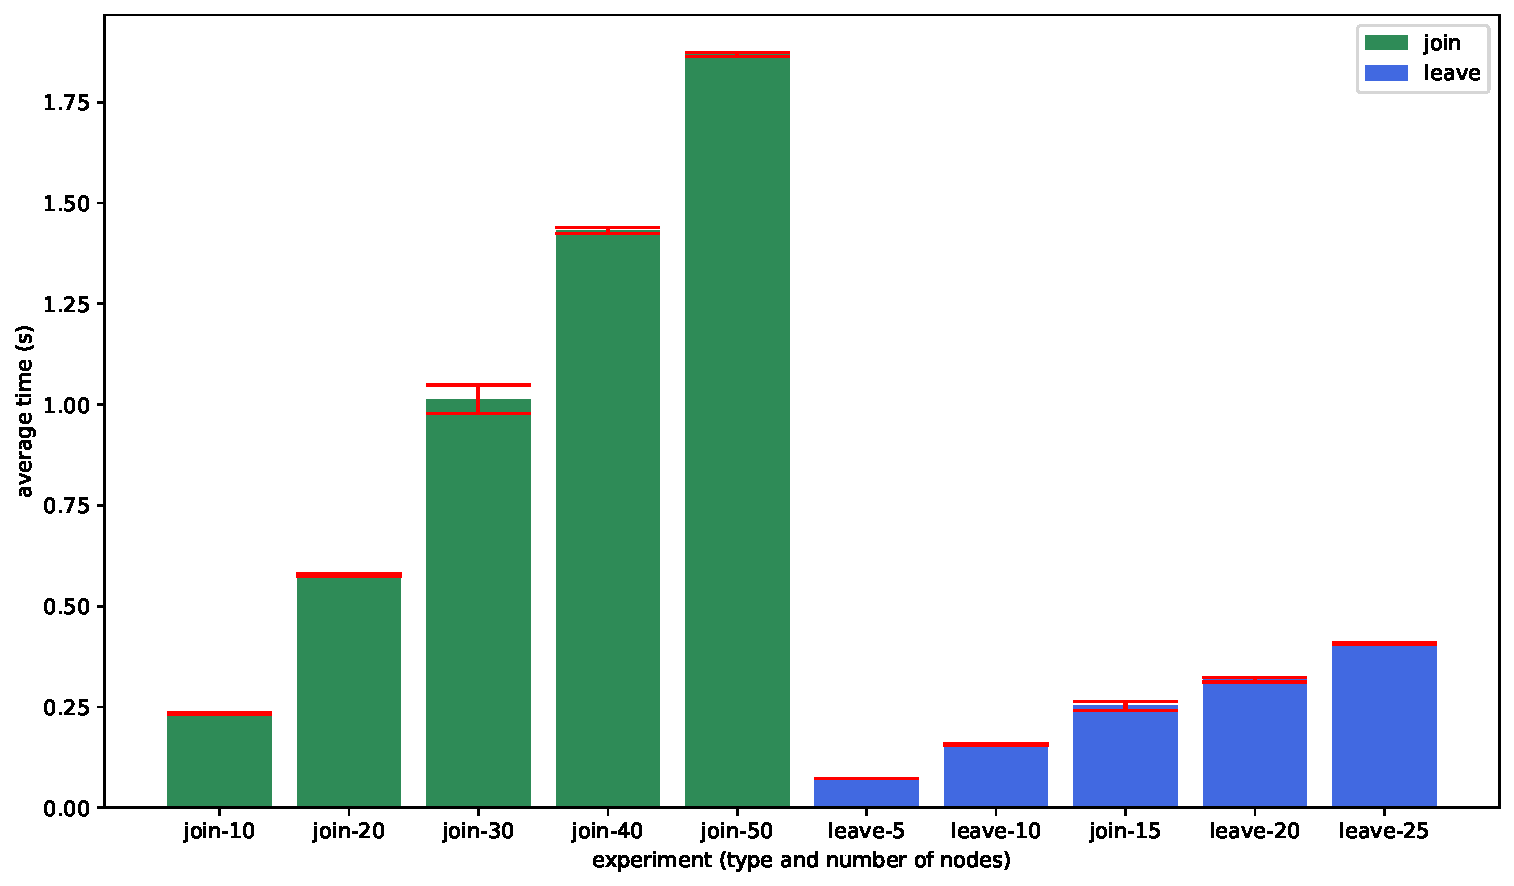
\includegraphics[width=7.5cm, height=5cm]{join_and_leave_bar.pdf}
	\caption{Histogram of average times for different nodes in experiment 1 and 2}
\end{figure}

Above graph implies that time to stabilize after a dynamic change (joining or leaving of nodes) in the network structure increases with number of nodes changed. This can be justified by the increase of requests passed among active nodes with the intention of adjusting the network structure. This overhead can be expected to be reduced if finger tables are used instead of adjacent neighbor communication as the lookup cost will be O(log$_2$n) thus minimizing the number of requests used.\\

Moreover, it was observed that a leave test scenario for the same number of nodes as a join, consumes only around a half of the latency of the join operation. This can be explained by the circulation of additional requests incurred by join procedure in finding the node's bucket space whereas node communicates directly and simultaneously with adjacent neighbors upon leaving.\\

Figure 2 illustrates the average times taken by experiment 3 for different number of crash nodes. Note that the adjusted latency is used in constructing the graph by reducing the detection timeout of 1 second in which a node will idly be waiting for a response.\\

\setlength{\intextsep}{10pt plus 2pt minus 0pt}
\begin{figure}[!ht]
	\centering
	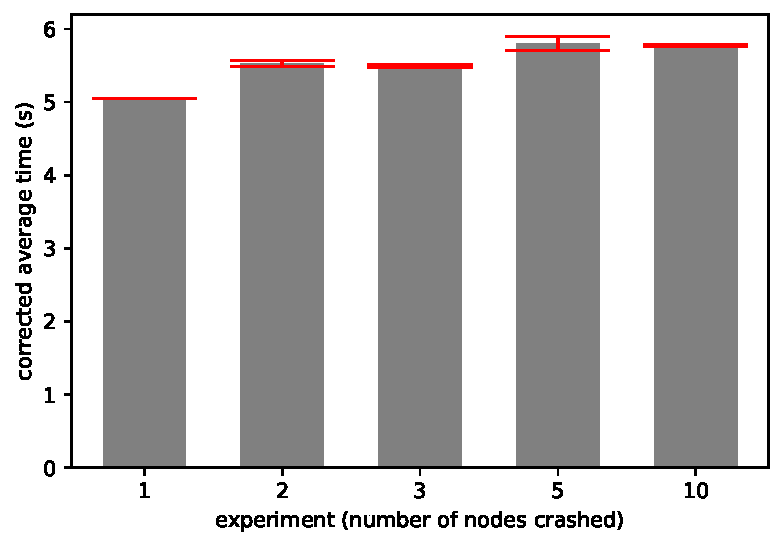
\includegraphics[width=7.5cm, height=5cm]{crash_bar.pdf}
	\caption{Histogram of corrected average times for different nodes in experiment 3}
\end{figure}

This graph shows that the implemented key-value store responds with a more or less time duration with a slightly increasing rate for different number of simultaneous crashes. Also it was observed that for higher number of crashes (preferably higher than 20), a few number of nodes had failed with elimination and re-establishment of the active nodes. This resulted in malfunctioning of a portion of partitioned networks while the rest had succeeded in rebuilding the connections.\\

Apart from them, additional experiments were carried out for the simultaneous recovery of the cluster after few crashes and it was observed that this mechanism leads to partitioned networks when \textit{/sim-recover} requests are sent in parallel. This observation can be explained as; by the time detection of a crashed node is corrected in the last active node of a partitioned network it may not be aware that a separate recovery is occurring in the adjacent network and hence lacks the communication between partitioned networks due to the implemented pull-based approach with timeouts. This could have been minimized if a push-based mechanism by the crashed node was used for recovery.

\section{Conclusion}

It is vital to address inconsistent nature of distributed systems as the existence of nodes can not be predicted. The implemented solution seems to be performing better with respect to this behavior. However it still possesses the disadvantage of passing HTTP requests all around the network since each node is only aware of its neighbors and even this can be improved with the integration of finger tables. 

\begin{thebibliography}{9}	
	\bibitem{chord}
	Ion Stoica, Robert Morris, David Karger, M. Frans Kaashoek, Hari Balakrishnan (2001) \emph{Chord: A Scalable Peer-to-Peer Lookup Service for Internet Applications }, MIT Laboratory for Computer Science.
	
	\bibitem{hash}
	A. L. Selvakumar and C. S. Ganadhas (2009) \emph{The Evaluation Report of SHA-256 Crypt Analysis Hash Function} International Conference on Communication Software and Networks.
	
	\bibitem{error}
	Lee, Dong and In, Junyong and Lee, Sangseok (2015) \emph{Standard deviation and standard error of the mean}, Korean journal of anesthesiology.
\end{thebibliography}

\appendix
\section{Source Code}
\href{https://github.com/YasiruR/dht/tree/master}{Github repository}

\end{document}
